\section{Zielsetzung}

%---------------------------------------------------------------------------------------------------------------------------------------------------------------%

\section{Theorie}
\subsection{Myonen}
% Standardmodell
% Lebensdauer
% Reichweite klassisch und relativistisch (E_\mu = \qty{10}{\GeV})

\subsection{Messung vom Szintillationsleuchten im Photodetektor}
% Szintillator
% Photodetektor


\subsection{Fehlerrechnung}
Für die Fehlerrechnung werden alle \textbf{Mittelwerte} von $N$ Messungen folgendermaßen berechnet:

\begin{equation}
    \overline{x} = \frac{1}{N} \cdot \sum_{i=1}^N x_i
    \label{eqn:Mittelwert}
\end{equation}

und alle \textbf{Standardabweichungen zum Mittelwert} mit:

\begin{equation}
    \increment\overline{x} = \sqrt{\frac{1}{N\cdot(N-1)}\cdot\sum_{i=1}^N (x_i-\overline{x})^2}
    \label{eqn:St_Mittelwert}
\end{equation}

Der Fehler für zusammenhängende Messwerte wird dann mit der \textbf{Gaußschen Fehlerfortpflanzung} berechnet:

\begin{equation}
    \increment{f} = \sqrt{ \sum_{i = 1}^{N}  \biggl(\frac{\partial{f}}{\partial{x_i}}\biggr)^2\cdot(\increment{x_i})^2}
    \label{eqn:Gauss}
\end{equation}

Die Fehlerfortpflanzung wird mit Uncertainties in Python \cite{uncertainties} ermittelt.

%---------------------------------------------------------------------------------------------------------------------------------------------------------------%

\section{Durchführung}
% Diskriminator mit variabler Schwelle

\begin{figure}
    \centering
    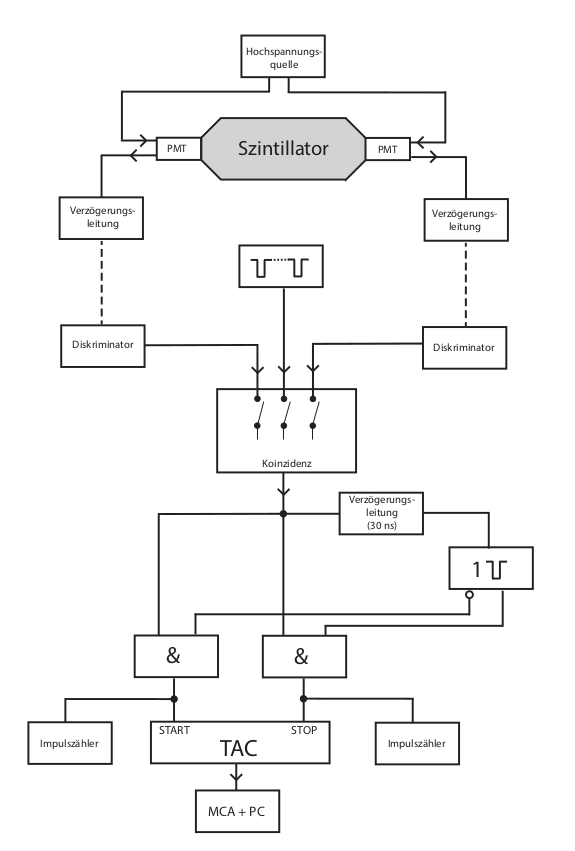
\includegraphics[width=0.8\textwidth]{./Bilder/aufbau.png}
    \caption{Blockschaltbild des Versuchsaufbaus}\label{fig:aufbau}
\end{figure}

In Abbildung \ref{fig:aufbau} ist der Aufbau abgebildet.
Der Szintillator Tank 